%! suppress = EscapeUnderscore
Topology is concerned with the properties of a geometric object that are preserved under continuous deformations,
such as stretching, twisting, crumpling and bending, but not tearing or gluing. \v

A topological space is a set endowed with a structure, called a topology, which allows defining continuous
deformation of subspaces, and, more generally, all kinds of continuity. Euclidean spaces, and, more generally, metric
spaces are examples of a topological space, as any distance or metric defines a topology. The deformations that are
considered in topology are homeomorphisms and homotopies. A property that is invariant under such deformations is a
topological property. Basic examples of topological properties are: the dimension, which allows distinguishing
between a line and a surface; compactness, which allows distinguishing between a line and a circle; connectedness,
which allows distinguishing a circle from two non-intersecting circles. \v

The ideas underlying topology go back to Gottfried Leibniz, who in the 17th century envisioned the geometria situs
and analysis situs. Leonhard Euler's Seven Bridges of Königsberg problem and polyhedron formula are arguably the
field's first theorems. The term topology was introduced by Johann Benedict Listing in the 19th century, although it
was not until the first decades of the 20th century that the idea of a topological space was developed.

\section{Topological Spaces}

We will now discuss topological spaces based on our previous development of axiomatic set theory. As we will see, a
topology on a set provides the weakest structure in order to define the two very important notions of convergence of
sequences to points in a set, and of continuity of maps between two sets. The definition of topology on a set is, at
first sight, rather abstract. But on the upside it is also extremely simple. This definition is the result of a
historical development, it is the simplest definition of topology that mathematician found to be useful.

\bd [Topology]
Let $M$ be a set. A \textbf{topology} on $M$ is a set $\cO \se \cP(M)$ such that:
\ben
\item[i)] $\vn \in \cO$ and $M \in \cO$.
\item[ii)] $\{U,V\}\se \cO \imp \bigcap\, \{U,V\} \in \cO$.
\item[iii)] $C \se \cO \imp \bigcup C \in \cO$.
\een
\ed

\bd [Topological Space]
Let $M$ be a set and $\cO$ a topology on the set $M$. The pair $(M,\cO)$ is called a \textbf{topological
space}. If we write ``let $M$ be a topological space'' then some topology $\cO$ on $M$ is
assumed.
\ed

Unless $|M|=1$, there are (usually many) different topologies $\cO$ that one can choose on the set $M$. The following
table summarizes the number of possible topologies (some of them might not satisfy the axioms, so they fail to be
topologies) given the cardinality of a set.
\btab[H]
\centering
\btb{c|c}
$|M|$ & \btb{@{}c@{}}Number of\\topologies\etb\\
\hline \rule{0pt}{12pt} 1 & 1 \\ 2 & 4 \\ 3 & 29 \\ 4 & 355 \\ 5 & 6,942 \\ 6 & 209,527 \\ 7 & 9,535,241 \\
\etb
\etab

\v

\be
Let $M = \{a,b,c\}$. Then $\cO=\{\vn,\{a\},\{b\},\{a,b\},\{a,b,c\}\}$ is a topology on $M$ since:
\ben
\item[i)] $\vn \in \cO$ and $M \in \cO$.
\item[ii)] Clearly, for any $S \in \cO$, $\bigcap\,\{\vn,S\}=\vn\in\cO$ and $\bigcap\,\{S,M\}=S\in\cO$. Moreover,
$\{a\}\cap\{b\}=\vn\in\cO$, $\ \{a\}\cap\{a,b\} =\{a\}\in \cO$, and $\{b\}\cap\{a,b\} =\{b\}\in \cO$.
\item[iii)] Let $C\se\cO$. If $M \in C$, then $\bigcup C = M\in \cO$. If $\{a,b\} \in C$ (or $\{a\},\{b\}\in C$) but
$M \notin C$, then $\bigcup C = \{a,b\}\in \cO$. If either $\{a\}\in C$ or $\{b\}\in C$, but $\{a,b\} \notin C$ and
$M \notin C$, then $\bigcup C = \{a\}\in \cO$ or $\bigcup C = \{b\}\in \cO$, respectively. Finally, if none of the
above hold, then $\bigcup C = \vn \in \cO$.
\een
\ee

\be
Let $M$ be a set. Then $\cO=\{\vn, M\}$ is a topology on $M$. Indeed, we have:
\ben
\item[i)] $\vn \in \cO$ and $M \in \cO$.
\item[ii)] $\bigcap\, \{\vn,\vn\} = \vn \in \cO$, $\ \bigcap\, \{\vn,M\} = \vn \in \cO$, and $\bigcap\, \{M,M\} = M \in \cO$.
\item[iii)] If $M \in C$, then $\bigcup C = M \in \cO$, otherwise $\bigcup C = \vn \in \cO$.
\een

This is called the \emph{chaotic topology} and can be defined on any set.
\ee

\be
Let $M$ be a set. Then $\cO=\cP(M)$ is a topology on $M$. Indeed, we have:
\ben
\item[i)] $\vn \in \cP(M)$ and $M \in \cP(M)$.
\item[ii)] If $U,V \in \cP(M)$, then $\bigcap\, \{U,V\} \se M$ and hence, $\bigcap\, \{U,V\} \in \cP(M)$.
\item[iii)] If $C\se\cP(M)$, then $\bigcup C \se M$, and hence, $\bigcup C\in \cP(M)$.
\een

This is called the \emph{discrete topology} and can be defined on any set.
\ee

We now give some common terminology regarding topologies.

\bd [Coarser / Finer Topology]
Let $\cO_1$ and $\cO_2$ be two topologies on a set $M$. If $\cO_1 \ss \cO_2$, then we say that $\cO_1$ is a
\textbf{coarser} (or \emph{weaker}) topology than $\cO_2$. Equivalently, we say that $\cO_2$ is a \textbf{finer} (or
\emph{stronger}) topology than $\cO_1$.
\ed

Clearly, the chaotic topology is the coarsest topology on any given set, while the discrete topology is the finest.

\bd [Open / Closed Subsets]
Let $(M,\cO)$ be a topological space. A subset $S$ of $M$ is said to be \textbf{open} (with respect to $\cO$) if $S
\in \cO$ and \textbf{closed} (with respect to $\cO$) if $M\sm S \in \cO$.
\ed

Notice that the notions of open and closed sets, as defined, are not mutually exclusive. A set could be either ``both or
neither'', or ``one and not the other''.

\be
Let $(M,\cO)$ be a topological space. Then $\vn$ is open since $\vn \in \cO$. However, $\vn$ is also closed since
$M\sm \vn = M \in \cO$. Similarly for $M$.
\ee

\be
Let $M = \{a,b,c\}$ and let $\cO=\{\vn,\{a\},\{a,b\},\{a,b,c\}\}$. Then $\{a\}$ is open but not closed, $\{b,c\}$ is
closed but not open, and $\{b\}$ is neither open nor closed.
\ee

We will now define what is called the standard topology on $\R^d$, where:
\bse
\R^d \coloneqq \underbrace{\R\times\R\times\cdots\times\R}_\text{$d$ times}
\ese

We will need the following auxiliary definition.

\bd [Open Balls]
For any $x\in\R^d$ and any $r \in \R^+ \coloneqq \{s\in\R\mid s>0\}$, we define the \textbf{open ball} of radius $r$
around the point $x$:
\bse
B_r(x) \coloneqq \bigl\{y\in \R^d \mid \textstyle\sqrt{\sum_{i=1}^d(y_i-x_i)^2} <r \bigr\}
\ese

\v

where $x \coloneqq (x_1,x_2,\ldots,x_d)$ and $y \coloneqq (y_1,y_2,\ldots,y_d)$, with $x_i,y_i\in\R$.
\ed

The quantity $\sqrt{\sum_{i=1}^d (y_i-x_i)^2}$ is usually denoted by $\|y-x\|_2$, where $\|\cdot\|_2$ is the 2-norm
on $\R^d$. However, the definition of a norm on a set requires the set to be equipped with a vector space structure
(which we haven't defined yet), while our construction does not. \v

Moreover, our construction can be proven to be independent of the particular norm used to define it, i.e.\ any other
norm will induce the same topological structure.

\bd [Standard Topology]
The \textbf{standard topology} on $\R^d$, denoted $\cO_\mathrm{std}$, is defined by:
\bse
U \in \cO_\mathrm{std} :\eqv \forall \, p \in U : \exists \, r \in \R^+ : B_r(p) \se U
\ese
\ed

Of course, simply calling something a topology, does not automatically make it into a topology. We have to prove that
$\cO_\mathrm{std}$ as we defined it, does constitute a topology. \v

This is actually a well known theorem.

\bt[]
The pair $(\R^d,\cO_\mathrm{std})$ is a topological space.
\et

Let's prove it!

\bq
\ben
\item[i)] First, we need to check whether $\vn \in \cO_\mathrm{std}$, i.e.\ whether is true:
\bse
\forall \, p \in \vn : \exists \, r \in \R^+ : B_r(p) \se \vn
\ese

This proposition is of the form $\forall \, p \in \vn : Q(p)$, which was defined as being equivalent to:
\bse
\forall \, p : p \in \vn \imp Q(p)
\ese

However, since $p\in\vn$ is false, the implication is true independent of $p$. Hence, the initial proposition is true
and thus $\vn \in \cO_\mathrm{std}$. \v

Second, by definition, we have $B_r(x)\se\R^d$ independent of $x$ and $r$, hence:
\bse
\forall \, p \in \R^d : \exists \, r \in \R^+ : B_r(p) \se \R^d
\ese

is true and thus $\R^d\in\cO_\mathrm{std}$.
\item[ii)] Let $U,V \in \cO_\mathrm{std}$ and let $p \in U \cap V$. Then:
\bse
p \in U \cap V :\eqv p \in U \land p \in V
\ese

and hence, since $U,V \in \cO_\mathrm{std}$, we have:
\bse
\exists \, r_1 \in \R^+ : B_{r_1}(p) \se U \quad \land \quad \exists \, r_2 \in \R^+ : B_{r_2}(p) \se V
\ese

Let $r=\min\{r_1,r_2\}$. Then:
\bse
B_r(p)\se B_{r_1}(p)\se U \quad \land \quad B_r(p)\se B_{r_2}(p)\se V
\ese

and hence, $B_r(p)\se U \cap V$. Therefore $U\cap V \in \cO_\mathrm{std}$.
\item[iii)] Let $C \se \cO_\mathrm{std}$ and let $p \in \bigcup C$. Then, $p\in U$ for some $U \in C$ and, since $U
\in \cO_\mathrm{std}$, we have:
\bse
\exists \, r \in \R^+ : B_r(p)\se U \se \bigcup C
\ese
\een

Therefore, $\cO_\mathrm{std}$ is indeed a topology on $\R^d$.
\eq

\section{Construction Of New Topologies From Given Ones}

One can construct new topologies from given ones. Here we will introduce the 3 most common ones which are:
\bit
\item Induced Topology.
\item Quotient Topology.
\item Product Topology.
\eit

Let's start with the ``induced topology''.

\bd [Induced Topology]
Let $(M,\cO)$ be a topological space and let $N\ss M$. Then we call the \textbf{induced topology} on $N$ the topology:
\bse
\cO|_N \coloneqq \{U\cap N \mid U \in \cO\} \se \cP(N)
\ese
\ed

Of course, we need to prove that this is indeed a topology.

\bq
\ben
\item[i)] Since $\vn \in \cO$ and $\vn = \vn \cap N$, we have $\vn \in \cO|_N$. Similarly, we have $M \in \cO$ and $N
= M \cap N$, and thus $N \in \cO|_N$.
\item[ii)] Let $U,V \in \cO|_N$. Then, by definition:
\bse
\exists \, S \in \cO : U = S \cap N \quad \land \quad \exists \, T \in \cO : V = T \cap N
\ese

We thus have:
\bse
U \cap V = (S\cap N) \cap (T \cap N) = (S\cap T) \cap N
\ese

\v

Since $S,T\in \cO$ and $\cO$ is a topology, we have $S\cap T \in \cO$ and hence, $U\cap V \in \cO|_N$.
\item[iii)] Let $C \coloneqq \{S_\a\mid \a \in \cA\} \se \cO|_N$. By definition, we have:
\bse
\forall \, \a \in \cA : \exists \, U_\a \in \cO : S_\a = U_\a \cap N
\ese

Then, using the notation:
\bse
\bigcup_{\a\in\cA}S_\a \coloneqq \bigcup C =\bigcup \,\{S_\a\mid \a \in \cA\}
\ese

and De Morgan's law, we have:
\bse
\bigcup_{\a\in\cA}S_\a = \bigcup_{\a\in\cA}(U_\a \cap N) = \bigg(\bigcup_{\a\in\cA}U_\a\biggr) \cap N
\ese

Since $\cO$ is a topology, we have $\bigcup_{\a\in\cA}U_\a \in \cO$ and hence, $\bigcup C \in \cO|_N$. \v

Thus, $\cO|_N$ is a topology on $N$.
\een
\eq

Let's see an example of an induced topology.

\be
Consider $(\R,\cO_\mathrm{std})$ and let:
\bse
N =[-1,1] \coloneqq \{x\in\R\mid -1 \leq x \leq 1\}
\ese

Then $(N,\cO_\mathrm{std}|_N)$ is a topological space. The set $(0,1]$ is clearly not open in $(\R,\cO_\mathrm{std})$
since $(0,1]\notin\cO_\mathrm{std}$. However, we have:
\bse
(0,1] = (0,2)\cap[-1,1]
\ese

\v

where $(0,2) \in \cO_\mathrm{std}$ and hence, $(0,1]\in\cO_\mathrm{std}|_N$, i.e.\ the set $(0,1]$ is open in $(N,
\cO_\mathrm{std}|_N)$.
\ee

Now let's define the ``quotient topology''.

\bd [Quotient Topology]
Let $(M,\cO)$ be a topological space and let $\sim$ be an equivalence relation on $M$. Then, the quotient set:
\bse
M/\!\sim \ = \{[m]\in \cP(M) \mid m \in M\}
\ese

\v

can be equipped with the \textbf{quotient topology} $\cO_{M/\sim}$defined by:
\bse
\cO_{M/\sim} \coloneqq \{U \in M/\!\sim \ \mid \bigcup U = \bigcup_{[a]\in U}[a] \in \cO \}
\ese
\ed

An equivalent definition of the quotient topology is as follows. Let $q\cl M \to M/\!\sim$ be the map:
\bi{rrCl}
q \cl & M & \to & M/\!\sim \\ & m & \mapsto & [m]
\ei

Then we have:
\bse
\cO_{M/\!\sim} \coloneqq \{U \in M/\!\sim \ \mid \mathrm{preim}_q(U) \in \cO \}
\ese

\v

\be
The \emph{circle} (or 1-sphere) is defined as the set $S^1 \coloneqq \{(x, y)\in \R^2\mid x^2+y^2=1\}$ equipped with
the subset topology inherited from $\R^2$. The open sets of the circle are (unions of) open arcs, i.e.\ arcs without
the endpoints. Individual points on the circle are clearly not open since there is no open set of $\R^2$ whose
intersection with the circle is a single point. However, an individual point on the circle is a closed set since its
complement is an open arc. \v

An alternative definition of the circle is the following. Let $\sim$ be the equivalence relation on $\R$ defined by:
\bse
x\sim y :\eqv \exists \, n \in \Z : x = y + 2\pi n
\ese

\v

Then the circle can be defined as the set $S^1 \coloneqq \R/\!\sim$ equipped with the quotient topology.
\ee

Finally, the ``product topology''.

\bd [Product Topology]
Let $(A,\cO_A)$ and $(B,\cO_B)$ be topological spaces. Then a topology on $A\times B$ is defined by the set
$\cO_{A\times B}$ called the \textbf{product topology} as:
\bse
U \in \cO_{A\times B} :\eqv \forall \, p \in U : \exists \, (S,T) \in \cO_A\times \cO_B : S\times T \se U
\ese
\ed

This definition can easily be extended to $n$-fold cartesian products:
\bse
U \in \cO_{A_1\times \cdots \times A_n} :\eqv \forall \, p \in U : \exists \, (S_1,\ldots,S_n) \in \cO_{A_1}\times
\cdots \times \cO_{A_n} : S_1\times \cdots\times S_n \se U
\ese

Using the previous definition, one can check that the standard topology on $\R^d$ satisfies:
\bse
\cO_\mathrm{std} = \cO_{\underbrace{\scriptstyle \R\times\R\times\cdots\times\R}_\text{ $d$ times}}
\ese

Therefore, a more minimalistic definition of the standard topology on $\R^d$ would consist in defining
$\cO_\mathrm{std}$ only for $\R$ (i.e.\ $d=1$) and then extending it to $\R^d$ by the product topology.

\section{Convergence \& Continuity}

\bd [Sequence]
Let $M$ be a set. A \textbf{sequence} (of points) in $M$ is a function $q \cl \N \to M$.
\ed

\bd [Convergence]
Let $(M,\cO)$ be a topological space. A sequence $q$ in $M$ is said to \textbf{converge} against a \emph{limit point}
$a\in M$ if:
\bse
\forall \, U \in \cO : a \in U \imp \exists \, N \in \N : \forall \, n > N : q(n) \in U
\ese
\ed

An open set $U$ of $M$ such that $a\in U$ is called an \emph{open neighbourhood} of $a$. If we denote this by $U(a)$,
then the previous definition of convergence can be rewritten as:
\bse
\forall \, U(a): \exists \, N \in \N : \forall \, n > N : q(n) \in U
\ese
\be

Consider the topological space $(M,\{\vn,M\})$. Then every sequence in $M$ converges to every point in $M$. Indeed,
let $q$ be any sequence and let $a \in M$. Then, $q$ converges against $a$ if:
\bse
\forall \, U \in \{\vn,M\} : a \in U \imp \exists \, N \in \N : \forall \, n > N : q(n) \in U
\ese

This proposition is vacuously true for $U=\vn$, while for $U=M$ we have $q (n)\in M$ independent of $n$. Therefore,
the (arbitrary) sequence $q$ converges to the (arbitrary) point $a\in M$.
\ee

\be
Consider the topological space $(M,\cP(M))$. Then only definitely constant sequences converge, where a sequence is
\emph{definitely constant} with value $c\in M$ if:
\bse
\exists \, N \in \N : \forall \, n > N : q(n) = c
\ese

This is immediate from the definition of convergence since in the discrete topology all singleton sets (i.e.\
one-element sets) are open.
\ee

\be
Consider the topological space $(\R^d,\cO_\mathrm{std})$. Then, a sequence $q\cl \N \to \R^d$ converges against $a\in
\R^d$ if:
\bse
\forall\, \ve >0 : \exists \, N \in \N : \forall \, n > N : \|q(n)-a\|_2<\ve
\ese
\ee

\v

\be
Let $M=\R$ and let $q=1-\frac{1}{n+1}$. Then, since $q$ is not definitely constant, it is not convergent in $(\R,\cP
(\R))$, but it is convergent in $(\R,\cO_\mathrm{std})$.
\ee

\bd [Continuity]
Let $(M,\cO_M)$ and $(N,\cO_N)$ be topological spaces and let $\phi\cl M\to N$ be a map. Then, $\phi$ is said to be
\textbf{continuous} (with respect to the topologies $\cO_M$ and $\cO_N$) if:
\bse
\forall \, S \in \cO_N \, , \ \mathrm{preim}_\phi(S) \in \cO_M
\ese

where $\mathrm{preim}_\phi(S) \coloneqq \{m \in M : \phi(m) \in S\}$ is the pre-image of $S$ under the map $\phi$.
\ed

Informally, one says that $\phi$ is continuous if the pre-images of open sets are open.

\be
If $M$ is equipped with the discrete topology, or $N$ with the chaotic topology, then any map $\phi\cl M \to N$ is
continuous. Indeed, let $S \in \cO_N$. If $\cO_M=\cP(M)$ (and $\cO_N$ is any topology), then we have:
\bse
\mathrm{preim}_\phi(S) = \{m \in M : \phi(m) \in S\} \se M \in \cP(M) = \cO_M
\ese

\v

If instead $\cO_N=\{\vn,N\}$ (and $\cO_M$ is any topology), then either $S=\vn$ or $S=N$ and thus, we have:
\bse
\mathrm{preim}_\phi(\vn) = \vn \in \cO_M \quad \t{and} \quad \mathrm{preim}_\phi(N) = M \in \cO_M
\ese
\ee

\be
Let $M = \{a,b,c\}$ and $N=\{1,2,3\}$, with respective topologies:
\bse
\cO_M=\{\vn,\{b\},\{a,c\},\{a,b,c\}\} \quad \t{and} \quad \cO_N=\{\vn,\{2\},\{3\},\{1,3\},\{2,3\},\{1,2,3\}\}
\ese

and let $\phi\cl M \to N$ by defined by:
\bse
\phi(a) = 2, \quad \phi(b)=1, \quad \phi(c)=2
\ese

Then $\phi$ is continuous. Indeed, we have:
\bse
\mathrm{preim}_\phi(\vn) = \vn, \:\:\: \mathrm{preim}_\phi(\{2\}) = \{a,c\}, \:\:\: \mathrm{preim}_\phi(\{3\}) = \vn, \:\:\: \mathrm{preim}_\phi(\{1,3\}) = \{b\},
\ese
\bse
\mathrm{preim}_\phi(\{2,3\}) = \{a,c\}, \:\:\: \mathrm{preim}_\phi(\{1,2,3\}) = \{a,b,c\}
\ese

and hence, $\mathrm{preim}_\phi(S) \in \cO_M$ for all $S \in \cO_N$.
\ee

\be
Consider $(\R^d,\cO_\mathrm{std})$ and $(\R^s,\cO_\mathrm{std})$. Then $\phi \cl \R^d\to\R^s$ is continuous with
respect to the standard topologies if it satisfies the usual $\ve$-$\delta$ definition of continuity:
\bse
\forall \, a \in \R^d: \forall \, \ve >0 :\exists \, \delta >0 : \forall \, 0<\|x-a\|_2<\delta:\|\phi(x)-\phi(a)\|_2<\ve
\ese
\ee

\bd [Homeomorphism]
Let $(M,\cO_M)$ and $(N,\cO_N)$ be topological spaces. A bijection $\phi\cl M\to N$ is called a
\textbf{homeomorphism} if both $\phi\cl M\to N$ and $\phi^{-1}\cl N\to M$ are continuous.
\ed

Homeo(morphism)s are the structure-preserving maps in topology. If there exists a homeomorphism $\phi$ between $(M,
\cO_M)$ and $(N,\cO_N)$:

\bse
\begin{tikzcd}
M \ar[rr, bend left,"\phi"] & & N \ar[ll, bend left,"\phi^{-1}"]
\end{tikzcd}
\ese

then $\phi$ provides a one-to-one pairing of the open sets of $M$ with the open sets of $N$.

\bd [Isomorphic Topological Spaces]
If there exists a homeomorphism between two topological spaces $(M,\cO_M)$ and $(N,\cO_N)$, we say that the two
spaces are \textbf{homeomorphic} or \textbf{topologically isomorphic} and we write $(M,\cO_M) \cong_\mathrm{top} (N,
\cO_N)$.
\ed

Clearly, if $(M,\cO_M) \cong_\mathrm{top} (N,\cO_N)$, then $M \iset N$.

\section{Invariant Topological Properties}

\bd [Invariant Topological Properties]
A property of a topological space is called an \textbf{invariant} if any two homeomorphic topological spaces share
the property.
\ed

In this section we will mention some of the (almost uncountable) invariant topological properties of topological
spaces. A \emph{classification} of topological spaces would be a list of topological invariants such that any two
spaces which share these invariants are homeomorphic. As of now, no such list is known!

\subsection{Separation Properties}

\bd [T1 Topological Space]
A topological space $(M,\cO)$ is said to be \textbf{T1} if for any two distinct points $p,q\in M$, $p\neq q$:
\bse
\exists \, U(p) \in \cO : q \notin U(p)
\ese
\ed

\bd [T2 or Hausdorff Topological Space]
A topological space $(M,\cO)$ is said to be \textbf{T2} or \textbf{Hausdorff} if, for any two distinct points, there
exist non-intersecting open neighbourhoods of these two points:
\bse
\forall \, p,q\in M : p\neq q \imp \exists \, U(p),V(q)\in \cO : U(p)\cap V(q) = \vn
\ese
\ed

\be
The topological space $(\R^d,\cO_\mathrm{std})$ is T2 and hence, also T1.
\ee

\be
The Zariski topology on an algebraic variety is T1 but not T2.
\ee

\be
The topological space $(M,\{\vn,M\})$ does not have the T1 property since for any $p \in M$, the only open
neighbourhood of $p$ is $M$ and for any other $q\neq p$ we have $q\in M$. Moreover, since this space is not T1, it
cannot be T2 either.
\ee

There are many other ``T'' properties, including a \emph{T2\sfrac{1}{2}} property which differs from T2 in that the
neighbourhoods are closed.

\bd [Cover]
Let $(M,\cO)$ be a topological space. A set $C \se \cP(M)$ is called a \textbf{cover} (of $M$) if:
\bse
\bigcup C = M
\ese

\v

Additionally, it is said to an \emph{open} cover if $C \se \cO$.
\ed

\bd [Open Cover]
Let $(M,\cO)$ be a topological space. A cover $C \se \cP(M)$ is said to be an \textbf{open cover} if $C \se \cO$.
\ed

\bd [Subcover]
Let $C$ be a cover. Then any subset $\widetilde{C}\se C$ such that $\widetilde{C}$ is still a cover, is called a
\textbf{subcover}. Additionally, it is said to be a \emph{finite} subcover if it is finite as a set.
\ed

\bd [Compact Topological Space]
A topological space $(M,\cO)$ is said to be \textbf{compact} if every open cover has a finite subcover.
\ed

\bd [Compact Subset]
Let $(M,\cO)$ be a topological space. A subset $N\se M$ is called \textbf{compact} if the topological space $(N,
\cO|_N)$ is compact.
\ed

Determining whether a set is compact or not is not an easy task. Fortunately though, for $\R^d$ equipped with the
standard topology $\cO_\mathrm{std}$, the following theorem greatly simplifies matters.

\bt[Heine-Borel]
Let $\R^d$ be equipped with the standard topology $\cO_\mathrm{std}$. Then, a subset of $\R^d$ is compact if, and
only if, it is closed and bounded.
\et

A subset $S$ of $\R^d$ is said to be \emph{bounded} if:
\bse
\exists \, r \in \R^+ : S \se B_r(0)
\ese

\be
The interval $[0,1]$ is compact in $(\R,\cO_\mathrm{std})$. The one-element set containing $(-1,2)$ is a cover of
$[0,1]$, but it is also a finite subcover and hence, $[0,1]$ is compact from the definition. Alternatively, $[0,1]$ is
clearly closed and bounded, and hence, it is compact by the Heine-Borel theorem.
\ee

\be
The set $\R$ is not compact in $(\R,\cO_\mathrm{std})$. To prove this, it suffices to show that there exists a cover
of $\R$ that does not have a finite subcover. To this end, let:
\bse
C \coloneqq \{(n,n+1)\mid n \in \Z\} \cup \{(n+\tfrac{1}{2}, n+\tfrac{3}{2})\mid n \in \Z\}
\ese

This corresponds to the following picture. \v

\begin{figure}[H]
\centering
\begin{tikzpicture}[scale=1.3]
\node (v2) at (4,0.5) {};
\node (v1) at (-4.75,0.5) {};
\draw (v1) edge (v2);
\draw [-triangle 60] (v1) edge (v2);
\node (v3) at (-4.5,1) {};
\node (v4) at (3.5,1) {};
\draw (v3) edge (v4);
\node (v5) at (-4.5,1.5) {};
\node (v6) at (3.5,1.5) {};
\draw (v5) edge (v6);
\draw[fill=white] (-0.5,1) circle (0.15);
\draw[fill=white] (-3.5,1) node (v7) {} circle (0.15);
\draw[fill=white] (2.5,1) circle (0.15);
\draw[fill=white] (-2,1.5) circle (0.15);
\draw[fill=white] (1,1.5) circle (0.15);
\draw (-3.5,0.62) edge (-3.5,0.38);
\draw (-2,0.62) edge (-2,0.38);
\draw (-0.5,0.62) edge (-0.5,0.38);
\draw (2.5,0.62) edge (2.5,0.38);
\draw (1,0.62) edge (1,0.38);
\node at (-3.5,0) {$-1$};
\node at (-2,0) {$-\sfrac{1}{2}$};
\node at (-0.5,0) {$0$};
\node at (1,0) {$\sfrac{1}{2}$};
\node at (2.5,0) {$1$};
\node at (3.7,0) {$\R$};
\node at (-4.8,1.22) {$C\ \Bigl\{$};
\end{tikzpicture}
\end{figure}

\v

It is clear that removing even one element from $C$ will cause $C$ to fail to be an open cover of $\R$. Therefore,
there is no finite subcover of $C$ and hence, $\R$ is not compact.
\ee

\bt[]
Let $(M,\cO_M)$ and $(N,\cO_N)$ be compact topological spaces. Then $ (M\times N,\cO_{M\times N})$ is a compact
topological space.
\et

The above theorem easily extends to finite cartesian products.

\bd [Refinement]
Let $(M,\cO)$ be a topological space and let $C$ be a cover. A \textbf{refinement} of $C$ is a cover $R$ such that:
\bse
\forall \, U \in R : \exists \, V \in C : U \se V
\ese
\ed

Any subcover of a cover is a refinement of that cover, but the converse is not true in general. A refinement $R$ is
said to be:
\bit
\item \emph{Open} if $R\se \cO$.
\item \emph{Locally finite} if for any $p\in M$ there exists a neighbourhood $U(p)$ such that the set:
\bse
\{U \in R \mid U \cap U(p) \neq \vn\}
\ese

is finite as a set.
\eit

Compactness is a very strong property. Hence, often times it does not hold, but a weaker and still useful property,
called paracompactness, may still hold.

\bd [Paracompact Topological Space]
A topological space $(M,\cO)$ is said to be \textbf{paracompact} if every open cover has an open refinement that is
locally finite.
\ed

\bt[]
If a topological space is compact, then it is also paracompact.
\et

Paracompactness is, informally, a rather natural property since every example of a non-paracompact space looks
artificial. One such example is the \emph{long line} (or \emph{Alexandroff line}). To construct it, we first observe
that we could ``build'' $\R$ by taking the interval $[0,1)$ and stacking countably many copies of it one after the
other. Hence, in a sense, $\R$ is equivalent to $\Z \times [0,1)$. The long line $L$ is defined analogously as
$L:\omega_1\times [0,1)$, where $\omega_1$ is an uncountably infinite set. The resulting space $L$ is not paracompact.

\bt[]
Let $(M,\cO_M)$ be a paracompact space and let $(N,\cO_N)$ be a compact space. Then $M\times N$ (equipped with the
product topology) is paracompact.
\et

\bt[]
Let $(M,\cO_M)$ be a paracompact space and let $(N_i,\cO_{N_i})$ be compact spaces for every $1\leq i \leq n$. Then
$M\times N_1\times\cdots\times N_n$ is paracompact.
\et

\bd [Partition Of Unity]
Let $(M,\cO_M)$ be a topological space. A \textbf{partition of unity} of $M$ is a set $\cF$ of continuous maps from
$M$ to the interval $[0,1]$ such that for each $p\in M$ the following conditions hold:
\ben
\item[i)] There exists $U(p)$ such that the set $\{f \in \cF \mid \forall \, x \in U(p):f(x)\neq 0\}$ is finite.
\item[ii)] $\sum_{f\in \cF}f(p)=1$.
\een

If $C$ is an open cover, then $\cF$ is said to be \emph{subordinate} to the cover $C$ if:
\bse
\forall \, f \in \cF : \exists \, U \in C : f(x) \neq 0 \imp x \in U
\ese
\ed

\bt[]
Let $(M,\cO_M)$ be a Hausdorff topological space. Then $(M,\cO_M)$ is paracompact if, and only if, every open cover
admits a partition of unity subordinate to that cover.
\et

\subsection{Connectedness \& Path-Connectedness}

\bd [Connected Topological Space]
A topological space $(M,\cO)$ is said to be \textbf{connected} unless there exist two non-empty, non-intersecting
open sets $A$ and $B$ such that $M=A\cup B$.
\ed

\be
Consider $(\R\sm \{0\},\cO_\mathrm{std}|_{\R\sm\{0\}})$, i.e.\ $\R\sm\{0\}$ equipped with the subset topology
inherited from $\R$. This topological space is not connected since $ (-\infty,0)$ and $(0,\infty)$ are open,
non-empty, non-intersecting sets such that $\R\sm\{0\}=(-\infty,0) \cup (0, \infty)$.
\ee

\bt[]
The interval $[0,1]\se\R$ equipped with the subset topology is connected.
\et

\bt[]
A topological space $(M,\cO)$ is connected if, and only if, the only subsets that are both open and closed are $\vn$
and $M$.
\et

\bd [Path - Connected Topological Space]
A topological space $(M,\cO)$ is said to be \textbf{path-connected} if for every pair of points $p,q\in M$ there
exists a continuous curve $\g\cl[0,1]\to M$ such that $\g(0)=p$ and $\g(1)=q$.
\ed

\be
The space $(\R^d,\cO_\mathrm{std})$ is path-connected. Indeed, let $p,q\in\R^d$ and let:
\bse
\g(\l) \coloneqq p+\l(q-p)
\ese

Then $\g$ is continuous and satisfies $\g(0)=p$ and $\g(1)=q$.
\ee

\be
Let $S \coloneqq \{(x,\sin(\tfrac{1}{x}))\mid x\in (0,1]\}\cup \{(0,0)\}$ be equipped with the subset topology
inherited from $\R^2$.

\fig{sinoneoverx}{0.19}

The space $(S,\cO_\mathrm{std}|_S)$ is connected but not path-connected.
\ee

\bt[]
If a topological space is path-connected, then it is also connected.
\et

\subsection{Homotopic Curves \& The Fundamental Group}

\bd [Homotopic Curves]
Let $(M,\cO)$ be a topological space. Two curves $\g,\delta\cl[0,1]\to M$ such that:
\bse
\g(0)=\delta(0) \quad \t{and} \quad \g(1)=\delta(1)
\ese

\v

are said to be \textbf{homotopic} if there exists a continuous map $h \cl [0,1]\times[0,1]\to M$ such that for all
$\l \in [0,1]$:
\bse
h(0,\l) = \g(\l) \quad \t{and} \quad h(1,\l)=\delta(\l)
\ese
\ed

Pictorially, two curves are homotopic if they can be continuously deformed into one another. \v

\begin{figure}[H]
\centering
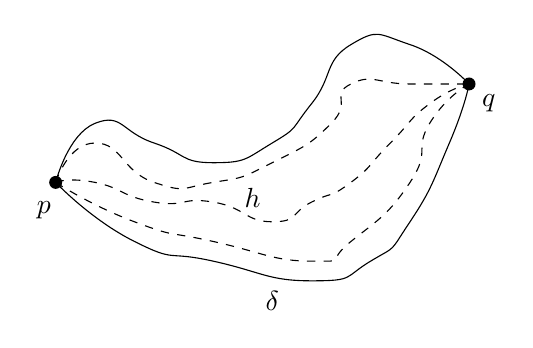
\begin{tikzpicture}[scale=0.5]
\draw plot[smooth, tension=.999] coordinates {(-3,-0.5) (-2,1) (-0.5,0.5) (1,0) (2.5,0.5) (3.5,1.5) (4.5,3) (6,3)
(7.5,2)};
\draw plot[smooth, tension=.999] coordinates {(-3,-0.5) (-1,-2) (1, -2.5) (3.5,-3) (5,-2.5) (6,-1.5) (7,0.5) (7.5,2)};
\draw[dashed] plot[smooth, tension=.999] coordinates {(-3,-0.5) (-2,0.5) (-0.5,-0.5) (1,-0.5) (2.5,0) (4,1) (4.5,2)
(6,2) (7.5,2)};
\draw[dashed] plot[smooth, tension=.999] coordinates {(-3,-0.5) (-2,-0.5) (-0.5,-1) (1,-1) (2.5,-1.5) (3.5, -1) (4.5,
-0.5) (5.5,0.5) (6.5,1.5) (7.5,2)};
\draw[dashed] plot[smooth, tension=.999] coordinates {(-3,-0.5) (-1,-1.5) (1,-2) (3.5,-2.5) (4.5,-2) (6,-0.5) (6.5,
1) (7.5,2)};
\draw[fill=black] (-3,-0.5) circle (0.15);
\draw[fill=black] (7.5,2) circle (0.15);
\node at (-3.3,-1.2) {$p$};
\node at (8,1.5) {$q$};
\node at (-1.5,1.5) {$\g$};
\node at (2,-0.9) {$h$};
\node at (2.5,-3.5) {$\delta$};
\end{tikzpicture}
\end{figure}

\v

\bt[]
Let $\g \sim \delta :\eqv$ ``$\g$ and $\delta$ are homotopic''. Then, $\sim$ is an equivalence relation.
\et

\bd [Space Of Loops]
Let $(M,\cO)$ be a topological space. Then, for every $p\in M$, we define the \textbf{space of loops} at $p$ by:
\bse
\mathscr{L}_p \coloneqq \{\g\cl[0,1]\to M \mid \g \t{ is continuous and } \g(0)=\g(1)\}
\ese
\ed

\bd [Concatenation]
Let $\mathscr{L}_p$ be the space of loops at $p\in M$. We define the \textbf{concatenation} operation $*\cl
\mathscr{L}_p\times\mathscr{L}_p\to\mathscr{L}_p$ by:
\bse
(\g * \delta) (\l) \coloneqq \left\{ \ba{ll} \g(2\l) & \t{if } 0\leq \l \leq \tfrac{1}{2}\\ \delta(2\l-1) & \t{if }
\tfrac{1}{2}\leq \l \leq 1 \ea \right.
\ese
\ed

\bd [Fundamental Group]
Let $(M,\cO)$ be a topological space. The \textbf{fundamental group} $\pi_1(p)$ of $(M,\cO)$ at $p\in M$ is the set:
\bse
\pi_1(p) \coloneqq \mathscr{L}_p/\!\sim\ = \{[\g] \mid \g \in \mathscr{L}_p\}
\ese

where $\sim$ is the homotopy equivalence relation, together with the map:
\bi{rrCl}
\bullet \cl & \pi_1(p)\times \pi_1(p) &\to &\pi_1(p)\\&(\g,\delta)&\mapsto & [\g]\bullet[\delta] \coloneqq [\g*\delta]
\ei
\ed

Observe that while all the previously discussed topological properties are ``boolean-valued'', i.e.\ a topological
space is either Hausdorff or not Hausdorff, either connected or not connected, and so on, the fundamental group is a
``group-valued'' property, i.e.\ the value of the property is not ``either yes or no'', but a group.

\be
The 2-sphere is defined as the set:
\bse
S^2 \coloneqq \{(x,y,z)\in \R^3\mid x^2+y^2+z^2=1\}
\ese

equipped with the subset topology inherited from $\R^3$.

\begin{center}
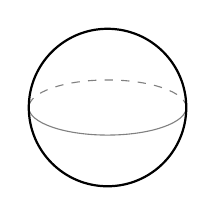
\begin{tikzpicture}[scale=0.5]
\draw[gray,dashed] (2,0) arc (0:180:2cm and 0.7cm);
\draw[gray] (2,0) arc (0:-180:2cm and 0.7cm);
\draw[thick] (0,0) circle[radius=2cm];
\end{tikzpicture}
\end{center}

The sphere has the property that all the loops at any point are homotopic, hence, the fundamental group (at every
point) of the sphere is the trivial group:
\bse
\forall \, p \in S^2 : \pi_1(p) = 1 \coloneqq \{[\g_e]\}
\ese
\ee

\be
The cylinder is defined as $C \coloneqq \R\times S^1$ equipped with the product topology.

\begin{center}
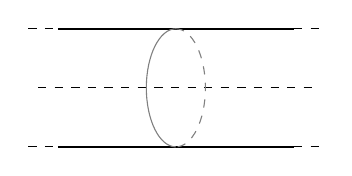
\begin{tikzpicture}[scale=0.5]
\draw[dashed] (-3.75,0) -- (-3,0);
\draw[dashed] (3,0) -- (3.75,0);
\draw[dashed] (-3.5,-1.5) -- (3.5,-1.5);
\draw[dashed] (-3.75,-3) -- (-3,-3);
\draw[dashed] (3,-3) -- (3.75,-3);
\draw[thick] (-3,0) -- (3,0);
\draw[thick] (-3,-3) -- (3,-3);
\draw[dashed,gray] (0,0) arc (90:-90:0.75cm and 1.5cm);
\draw[gray] (0,0) arc (90:270:0.75cm and 1.5cm);
\end{tikzpicture}
\end{center}

A loop in $C$ can either go around the cylinder (i.e.\ around its central axis) or not. If it does not, then it can
be continuously deformed to a point (the identity loop). If it does, then it cannot be deformed to the identity loop
(intuitively because the cylinder is infinitely long) and hence, it is a homotopically different loop. The number of
times a loop winds around the cylinder is called the \emph{winding number}. Loops with different winding numbers are
not homotopic. \v

Moreover, loops with different \emph{orientations} are also not homotopic and hence, we have:
\bse
\forall \, p \in C : (\pi_1(p),\bullet) \cong_\mathrm{grp}(\Z,+)
\ese
\ee

\be
The 2-torus is defined as the set $T^2 \coloneqq S^1\times S^1$ equipped with the product topology.

\begin{center}
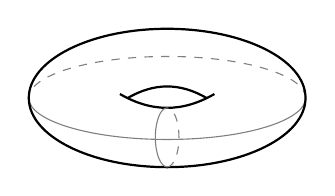
\begin{tikzpicture}[scale=0.5]
\draw[thick] (-1,0) to[bend left] (1,0);
\draw[thick] (-1.2,.1) to[bend right] (1.2,.1);
\draw[gray] (100pt,0) arc (0:-180:100pt and 30pt);
\draw[gray,dashed] (100pt,0) arc (0:180:100pt and 30pt);
\draw[thick] (0,0) ellipse (100pt and 50pt);
\draw[gray,dashed] (0,-1.75) arc (-90:90:0.3 and 0.75);
\draw[gray] (0,-1.75) arc (-90:-270:0.3 and 0.75);
\end{tikzpicture}
\end{center}

A loop in $T^2$ can intuitively wind around the cylinder-like part of the torus as well as around the hole of the
torus. That is, there are two independent winding numbers and hence:
\bse
\forall \, p \in T^2 : \pi_1(p) \cong_\mathrm{grp}\Z\times \Z
\ese

where $\Z\times \Z$ is understood as a group under pairwise addition.
\ee